\documentclass[../thesis]{subfiles}

\begin{document}

\chapter{Architecture}
Characterization and development of sensor arrays presents a broad
range of research challenges, not least of which relate to data
organization. A \gls{LIMS} adequate to the needs of our example
application must provide a number of interacting software components
to mediate between users and target resources such as data stores,
richly featured research documents, computer-controllable lab
equipment, and collaborators. This chapter abstractly describes the
constituent components of the software framework we have built for
collaborative design, execution, and analysis of experiments. When
describing each element, we document some of the phases of our
iterative design process that led to these decisions.

\section{Network architecture}
Given that the resources of interest to our software system are
inherently distributed, a careful design of the system's network
interconnections is critical to its scalability, security, and
usefulness. Below we describe the physical system constraints driving
some of our design decisions and explain how we iteratively arrived at
our final design.

\subsection{Physical architecture}
Typical workflows for interdisciplinary digital research involve a
number of computing resources which are physically and logically
separated from each other. These include (i) individual workstations
where researchers perform analysis and compose code and documentation,
(ii) intranet and cloud storage drives for archiving and sharing
documents and data, (iii) logs of research-relevant communications
such as email correspondence, and (iv) dedicated, typically shared
scientific resources such as lab instruments and high-performance
computers. In many cases, especially in electrical engineering, a
device we generically categorize as a piece of ``lab equipment'' is a
focus of research in its own right, and can be further decomposed to
include computer controllers, instrumentation electronics, and
physical processes or devices of interest. Often some or all of these
resources interact with each other in an ad-hoc fashion manually
facilitated by users. We believe that tremendous gains can be made for
research organization, accuracy, and reproducibility by coordinating
the interactions between these components with a carefully designed
software framework. A schematic diagram of some of these interacting
components is depicted in figure \ref{fig:PhysArch}.

\begin{figure}
  % \includegraphics[width=\textwidth]{phys-arch}
  \caption{
    Representation of some of the digital resources found in typical
    scientific workflows and their relationships.
    \label{fig:PhysArch}
  }
\end{figure}

The most important goal of the present work is to automatically
execute physical experiments by employing computer control,
automatically collating raw experimental data with secondary data and
metadata to produce self-contained research artifacts that are more
amenable to unambiguous analysis than present ad-hoc formats.
Ideally we would like for collaborating researchers at different
universities to be able to review each others' experiments in real
time, allowing for continuous feedback between investigators with
different areas of expertise.

Although some pieces of modern lab equipment possess network interfaces
and can directly act as web servers in their own right, a majority of
scientific instruments of interest operate over short-range or legacy
communication links. In order to allow users to remotely interact with
physical resources of this kind, at least one additional machine is
required. This machine is typically represented by a PC physically
located in a research lab and connected directly to external hardware
devices over non-networked connections such as USB.

\subsection{Monolithic approach}
\begin{figure}
  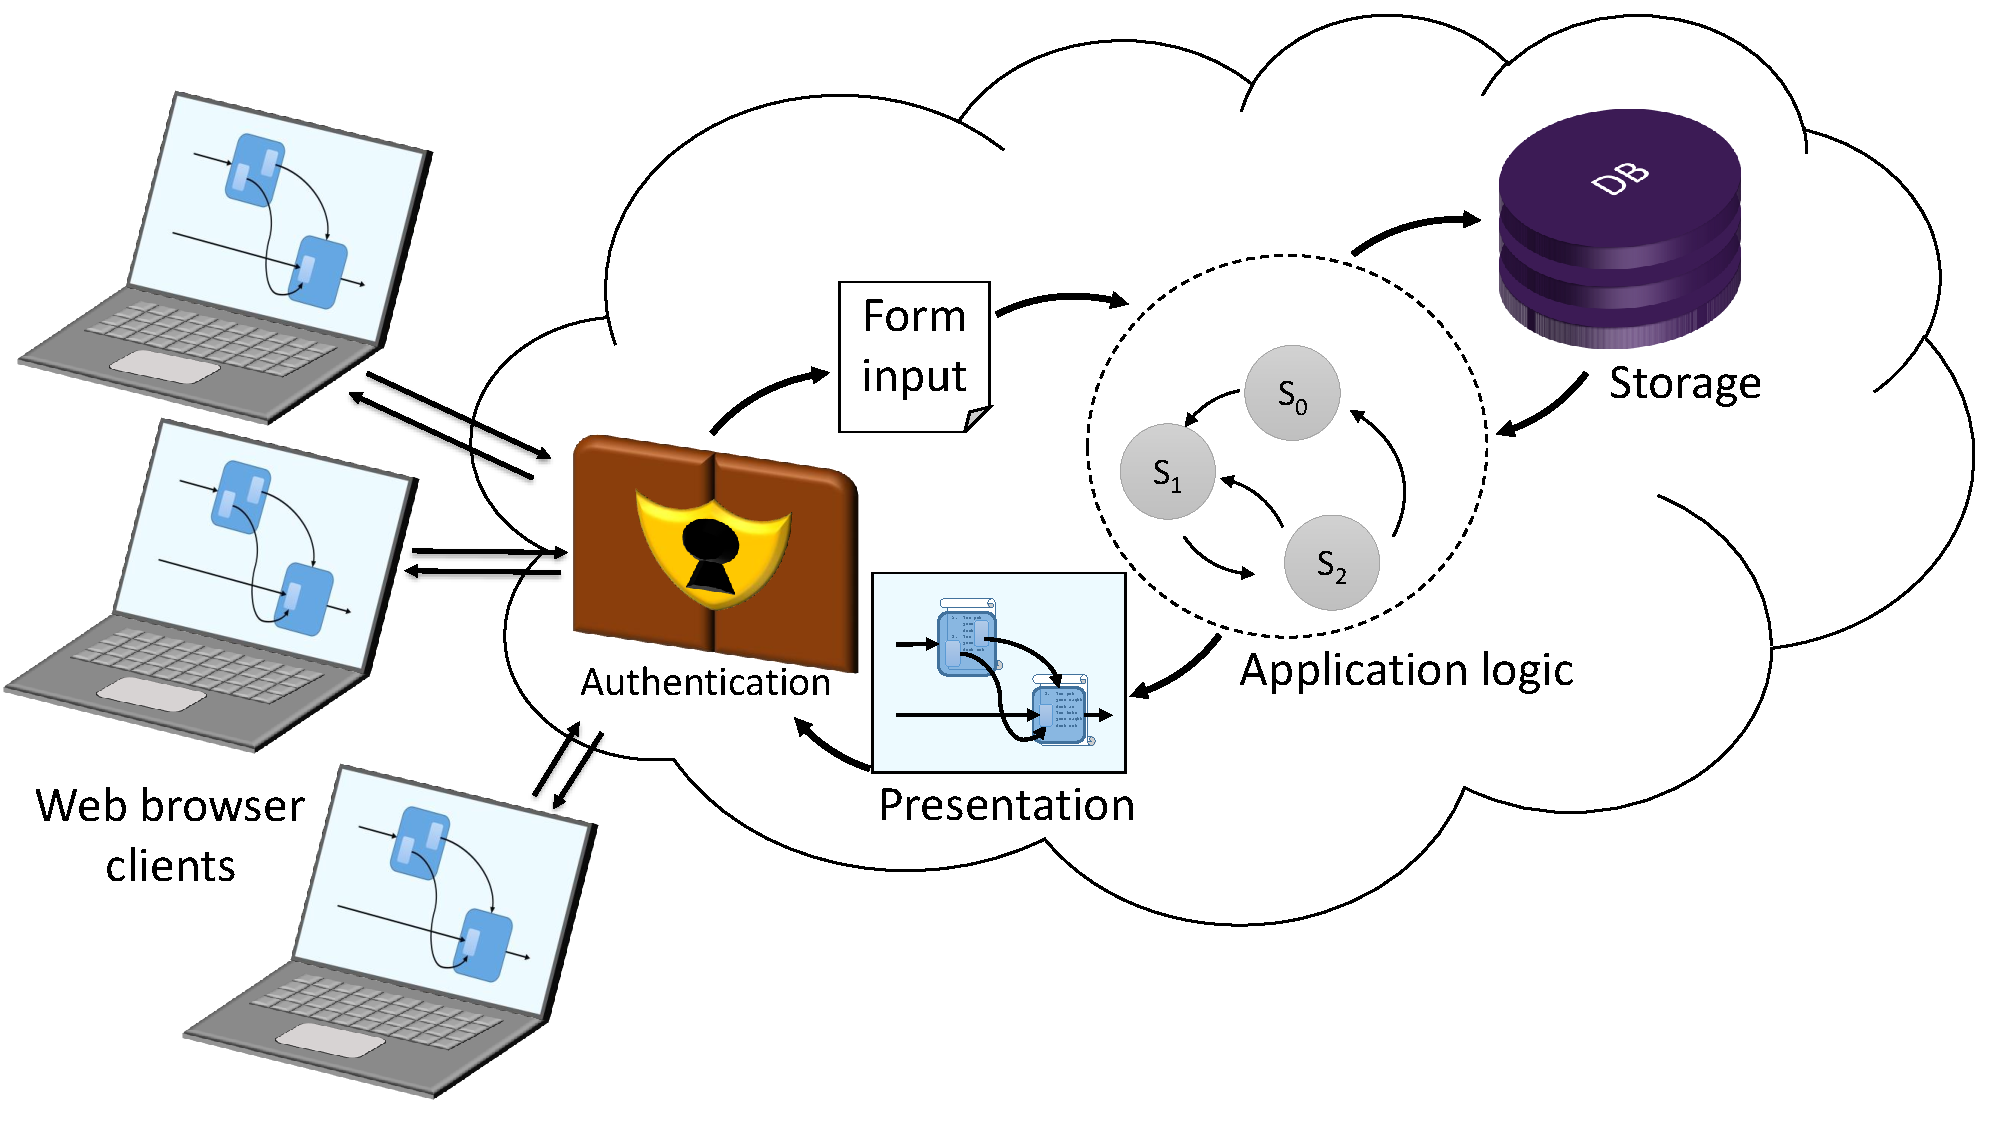
\includegraphics[width=\textwidth]{monolithic}
  \caption{
    A traditional ``monolithic'' web application architecture where
    one server process manipulates a database on behalf of many clients.
    \label{fig:Monolithic}
  }
\end{figure}

A traditional architecture for web application software involves a
single server executable serving presentation-layer applications to
clients and making database accesses on their behalf, as in figure
\ref{fig:Monolithic}. In our case, the server would also mediate
access to lab equipment, providing users with indirect and high-level
access to these resources in much the same way as it abstracts over
the database.

This architecture is attractive for its ease of deployment and its
apparent simplicity, and early in the project's development we pursued
a design along these lines. However, attempting to bundle all of the
system's server-side functionality into a single program eventually
caused difficulty with system integration. For example, coupling the
code for communicating with lab instruments into the server's
application logic complicates both portions of the program and makes
it difficult to test and develop them in isolation. This agrees with a
common observation \cite{Stephens:2015:BSE:2826034} that architectures
of this kind are often less modular, making them more difficult for
multiple programmers to develop independently and complicating the
process of introducing new functionality. We feel that a more
compartmentalized, modular approach better reflects the structure of
the domain being modeled as well as conferring a number of software
engineering benefits.

\subsection{Microservices}
As opposed to the conventional \gls{frontend}-\gls{backend} divide, some
developers have suggested an architecture for web applications based
on simple communicating modules termed \glspl{microservice}. In a
traditional monolithic architecture, programmers compose a complicated
application hierarchically, using one main module which calls library
functions from many subordinate components.  A microservice
architecture splits functionality into many independent programs which
communicate using ordinary network protocols, and modules are designed
to assume that their dependencies are completely separate programs
potentially running on other machines \cite{Micro14:online}.  This
approach promises better modularity than traditional web applications
since capabilities can be added and extended independently of one
another \cite{Balalaie2016}. Since all services expose their
functionality over a similar web \gls{API}, implementations are
decoupled from each other and internally have very different
architectures tailored to their special-purpose needs.  Services may
even be written in completely different programming languages. The
flexibility that this approach affords is a good fit with our desire
to adapt the framework to meet users' changing needs. Furthermore, a
microservice architecture lends itself naturally to a design where
capabilities and resources are distributed geographically, as is the
case with large, remotely collaborating groups of researchers. In some
cases microservice architectures also scale better as performance
demands on the system increase \cite{}.

\begin{figure}
  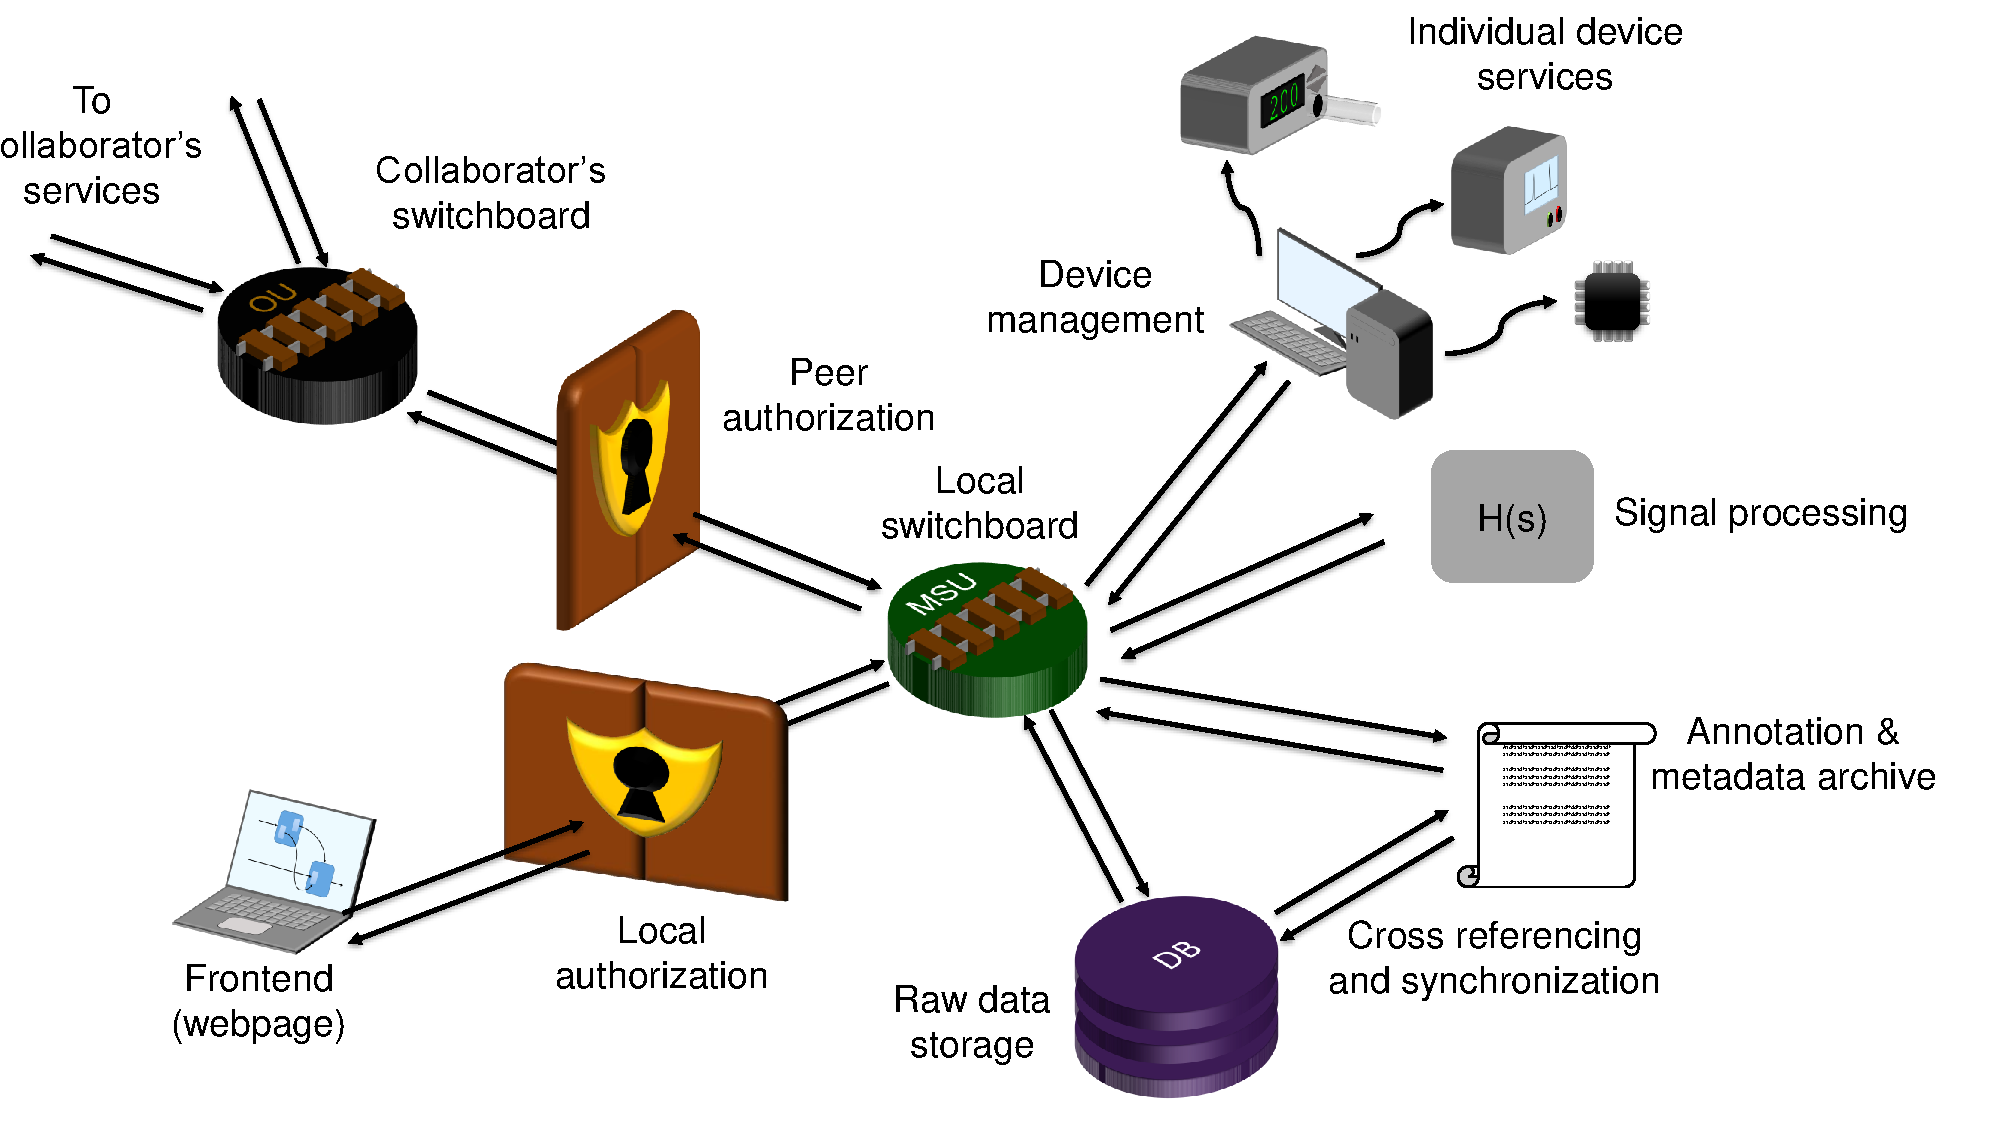
\includegraphics[width=\textwidth]{microservices}
  \caption{
    High-level interconnection between the critical microservices
    composing our final design.
    \label{fig:Microservices}
  }
\end{figure}

A schematic depicting the connections between some of our core
microservices can be found in figure \ref{fig:Microservices}.

\subsection{Switchboard service}
Despite its internally distributed design, the web application must
present a primary gateway for user interaction. In our design this
role is taken by a microservice we refer to as a \gls{switchboard}

\section{Device control}
A core goal of our design is to enable researchers to incorporate
choreography of physical lab equipment into the executable workflows
they create. Interacting with the variety of commercial and custom
hardware found in a typical experimental lab requires a flexible
approach, given that computer control interfaces and data formats for
scientific equipment are heterogeneous and very poorly
standardized. This section describes an approach for building a
modular library of device drivers which integrate with the rest of the
system while providing users with tools for extension and
customization.

\subsection{Instrument manager}
The instrument manager is a microservice responsible for detecting
connected devices, determining the appropriate device driver for
communicating with them, and presenting a unified interface to the
switchboard.

\subsection{Interface API}

\subsection{Enumeration}

\subsection{Protocol composition}



\section{Data model}

\subsection{entity models}

\subsection{dataset tabulation}



\section{User experience}



\section{Security}



\end{document}
